
\section{Pipe system}


Our {\em Diff} model is not only accurate for classification. It can also provide upper bounds on the output of DNN-regressor due to small perturbations of the input.
We consider here a pipe system and its DNN regressor from \cite{aiware},
that predicts the plastic strain in 3000 points of a mesh over a pipe given the deformation of each of these 3000 points.
Compared to the classification tasks where the DNN is learned in a standard way and PCA is later applied to reduce the output dimension without compromising the accuracy, the DNN regressor has been learned on the reduced PCA basis directly, for both the high dimensional input and the high dimensional output (3000 dimensions each).



\begin{figure*}[t!]
	\centering
	
\includegraphics[scale=0.6]{PIPE.pdf} 
	\vspace{-0.5cm}
	\caption{Training and bound computation on the pipe use case. 
		Two PCAs are used, for the input (deformation) and for the output space (plastic strain). The surrogate is learned from reduced deformation input to reduced strain output.}
	\vspace{-0.2cm}
	\label{fig.PIPE}
\end{figure*}	


Figure \ref{fig.PIPE} describes the pipeline used to learn the DNN regressor for the pipe system. The DNN that has been learned has 2 fully connected layers, 50 neurons each, learned as a surrogate model, with 10 reduced input and 26 reduced output.

In terms of perturbation, a conjunction of $L_1 \leq 3.9$ and $L_\infty \leq .02$ perturbations, physically pertinent dimensions, and maximizes the sum of the difference in output of 10 selected points in the mesh between input and its deformation.



\begin{table}[b!]
	\centering
	\begin{tabular}{|c | c c c c c|} 
		\hline
		Pipe & Timeout & ITNE & {\em Diff} & {\em 2$b+$1} & {\em 1$b$}
		\\\hline 
		& 1000s & 0.045 & 0.042 & 0.041 & {\bf 0.036}
		\\
		Surrogate  & 14400s & 0.042 & 0.036 & {\bf 0.035} & 0.036
		\\
		LB = $.025$  & 72000s & 0.042 & 0.034 & {\bf 0.033} & 0.036
		\\\hline
	\end{tabular}
	\caption{Comparison of upper bound (lower is better $\downarrow$) between {\em Diff}, {\em 2$b+$1}, {\em 1$b$} with ITNE on the pipe system with timeouts of 1000s, 14440s and 72000s.}
	%L1 corresponds to $3.9$ or $4$, and results should be the sum of 10 pixels, so around 10 times higher values.}
\label{table.pipe}
\end{table}


\begin{figure*}[t!]
\centering
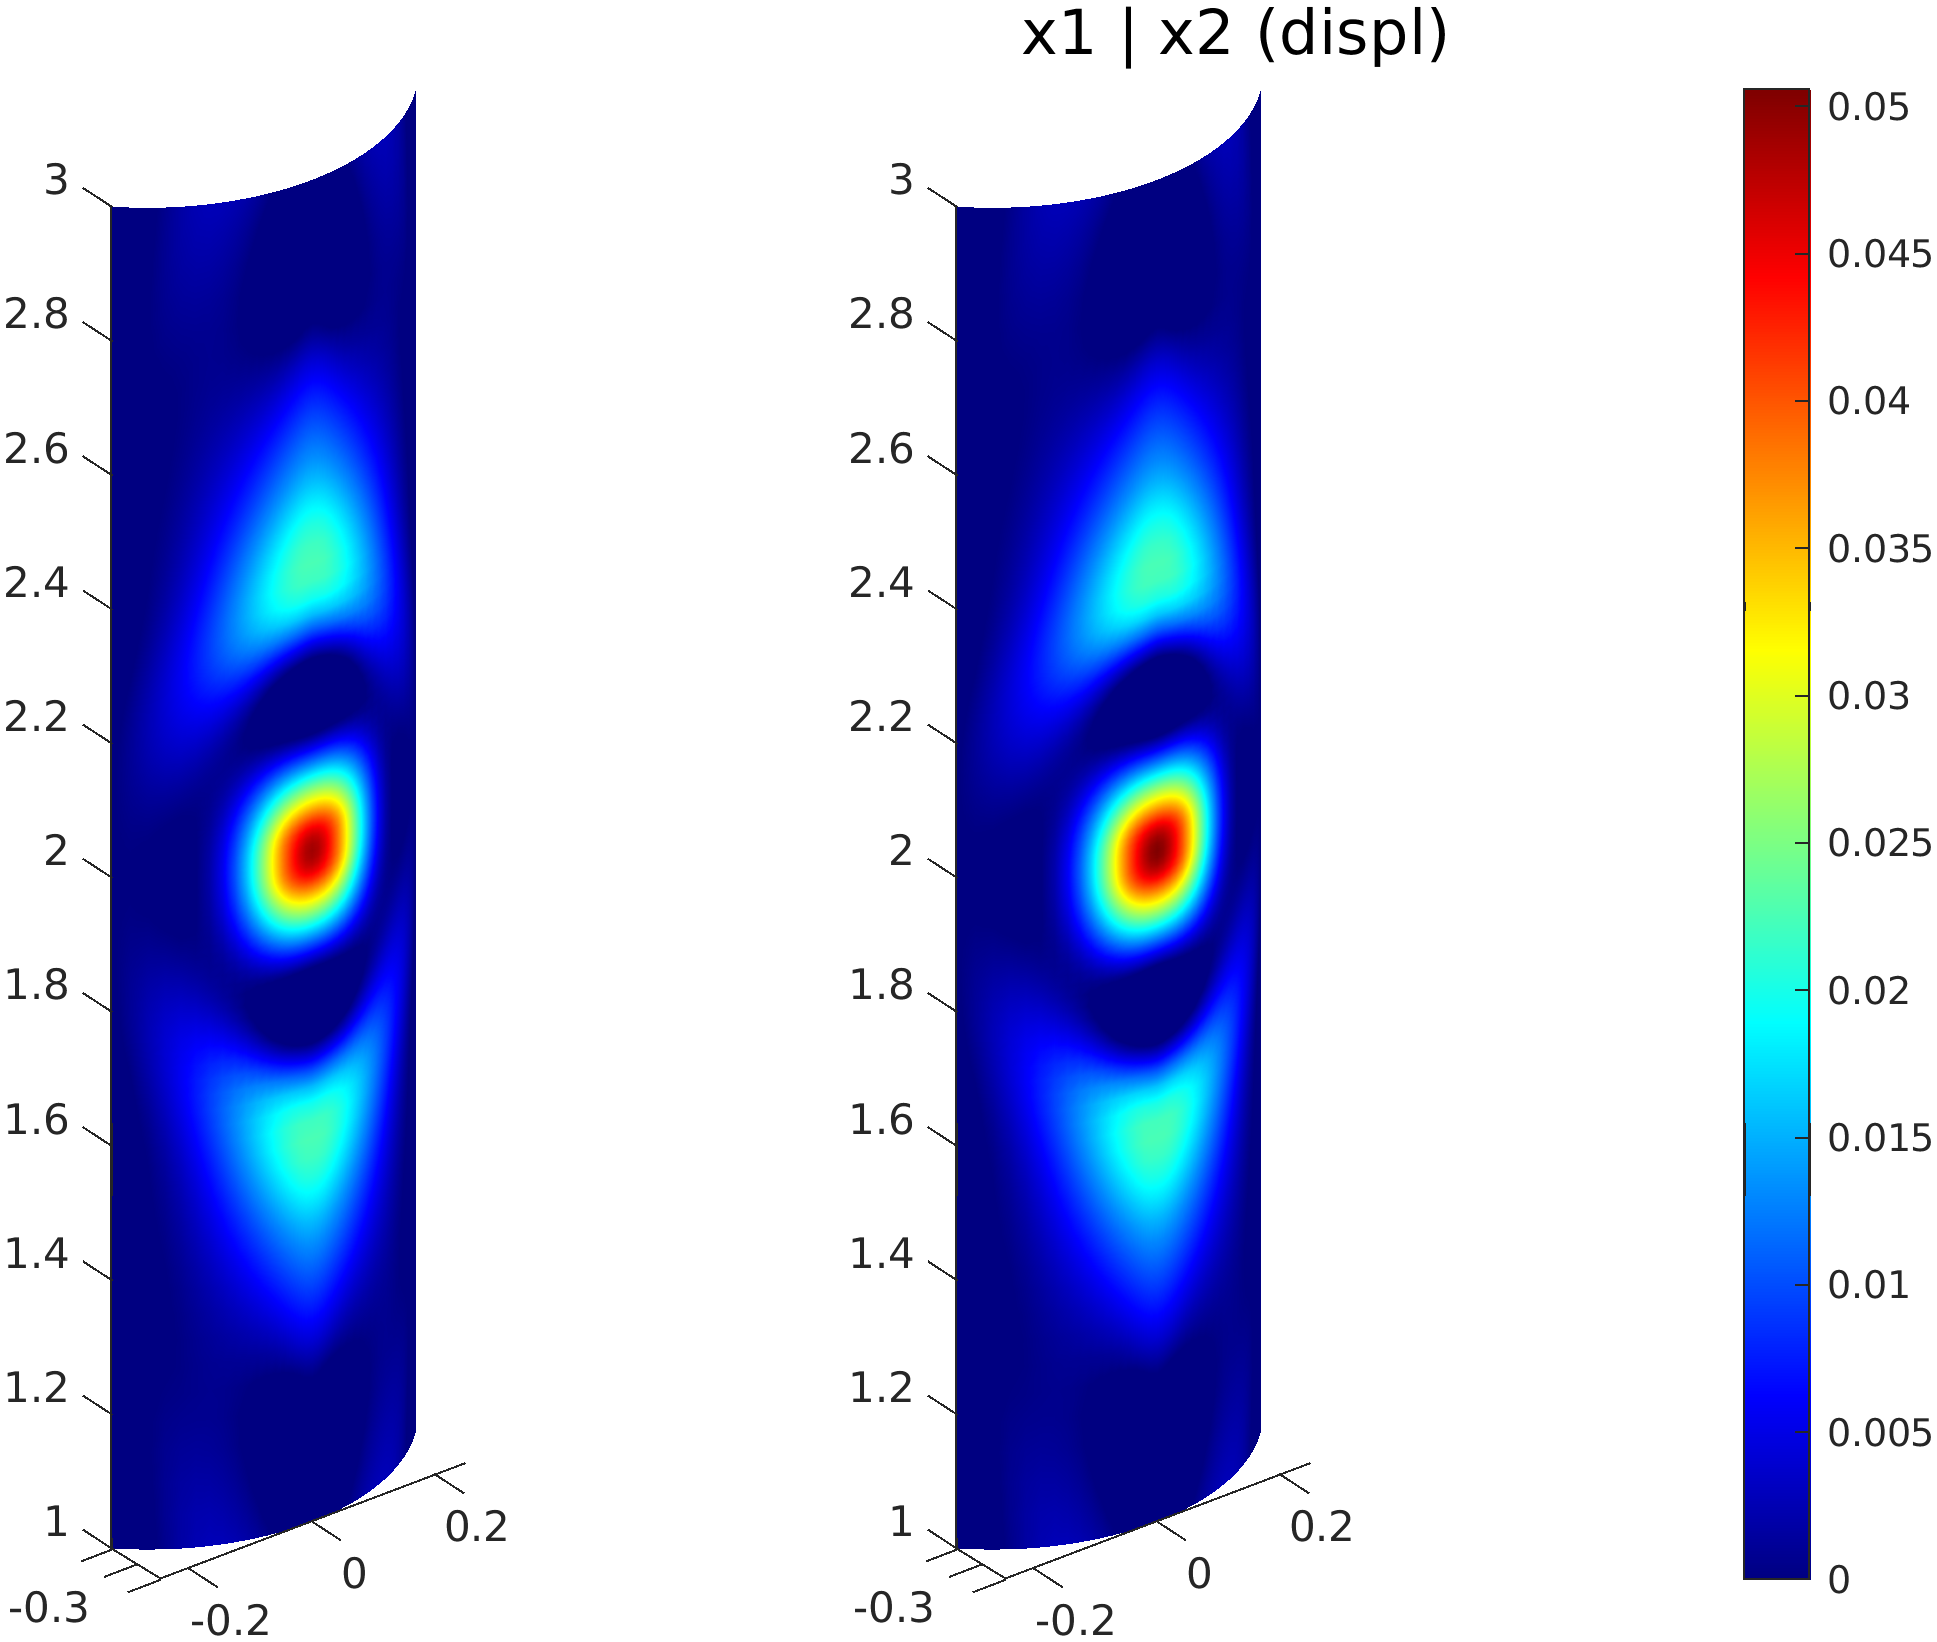
\includegraphics[scale=0.36]{deform.png} \hspace{0.1cm}
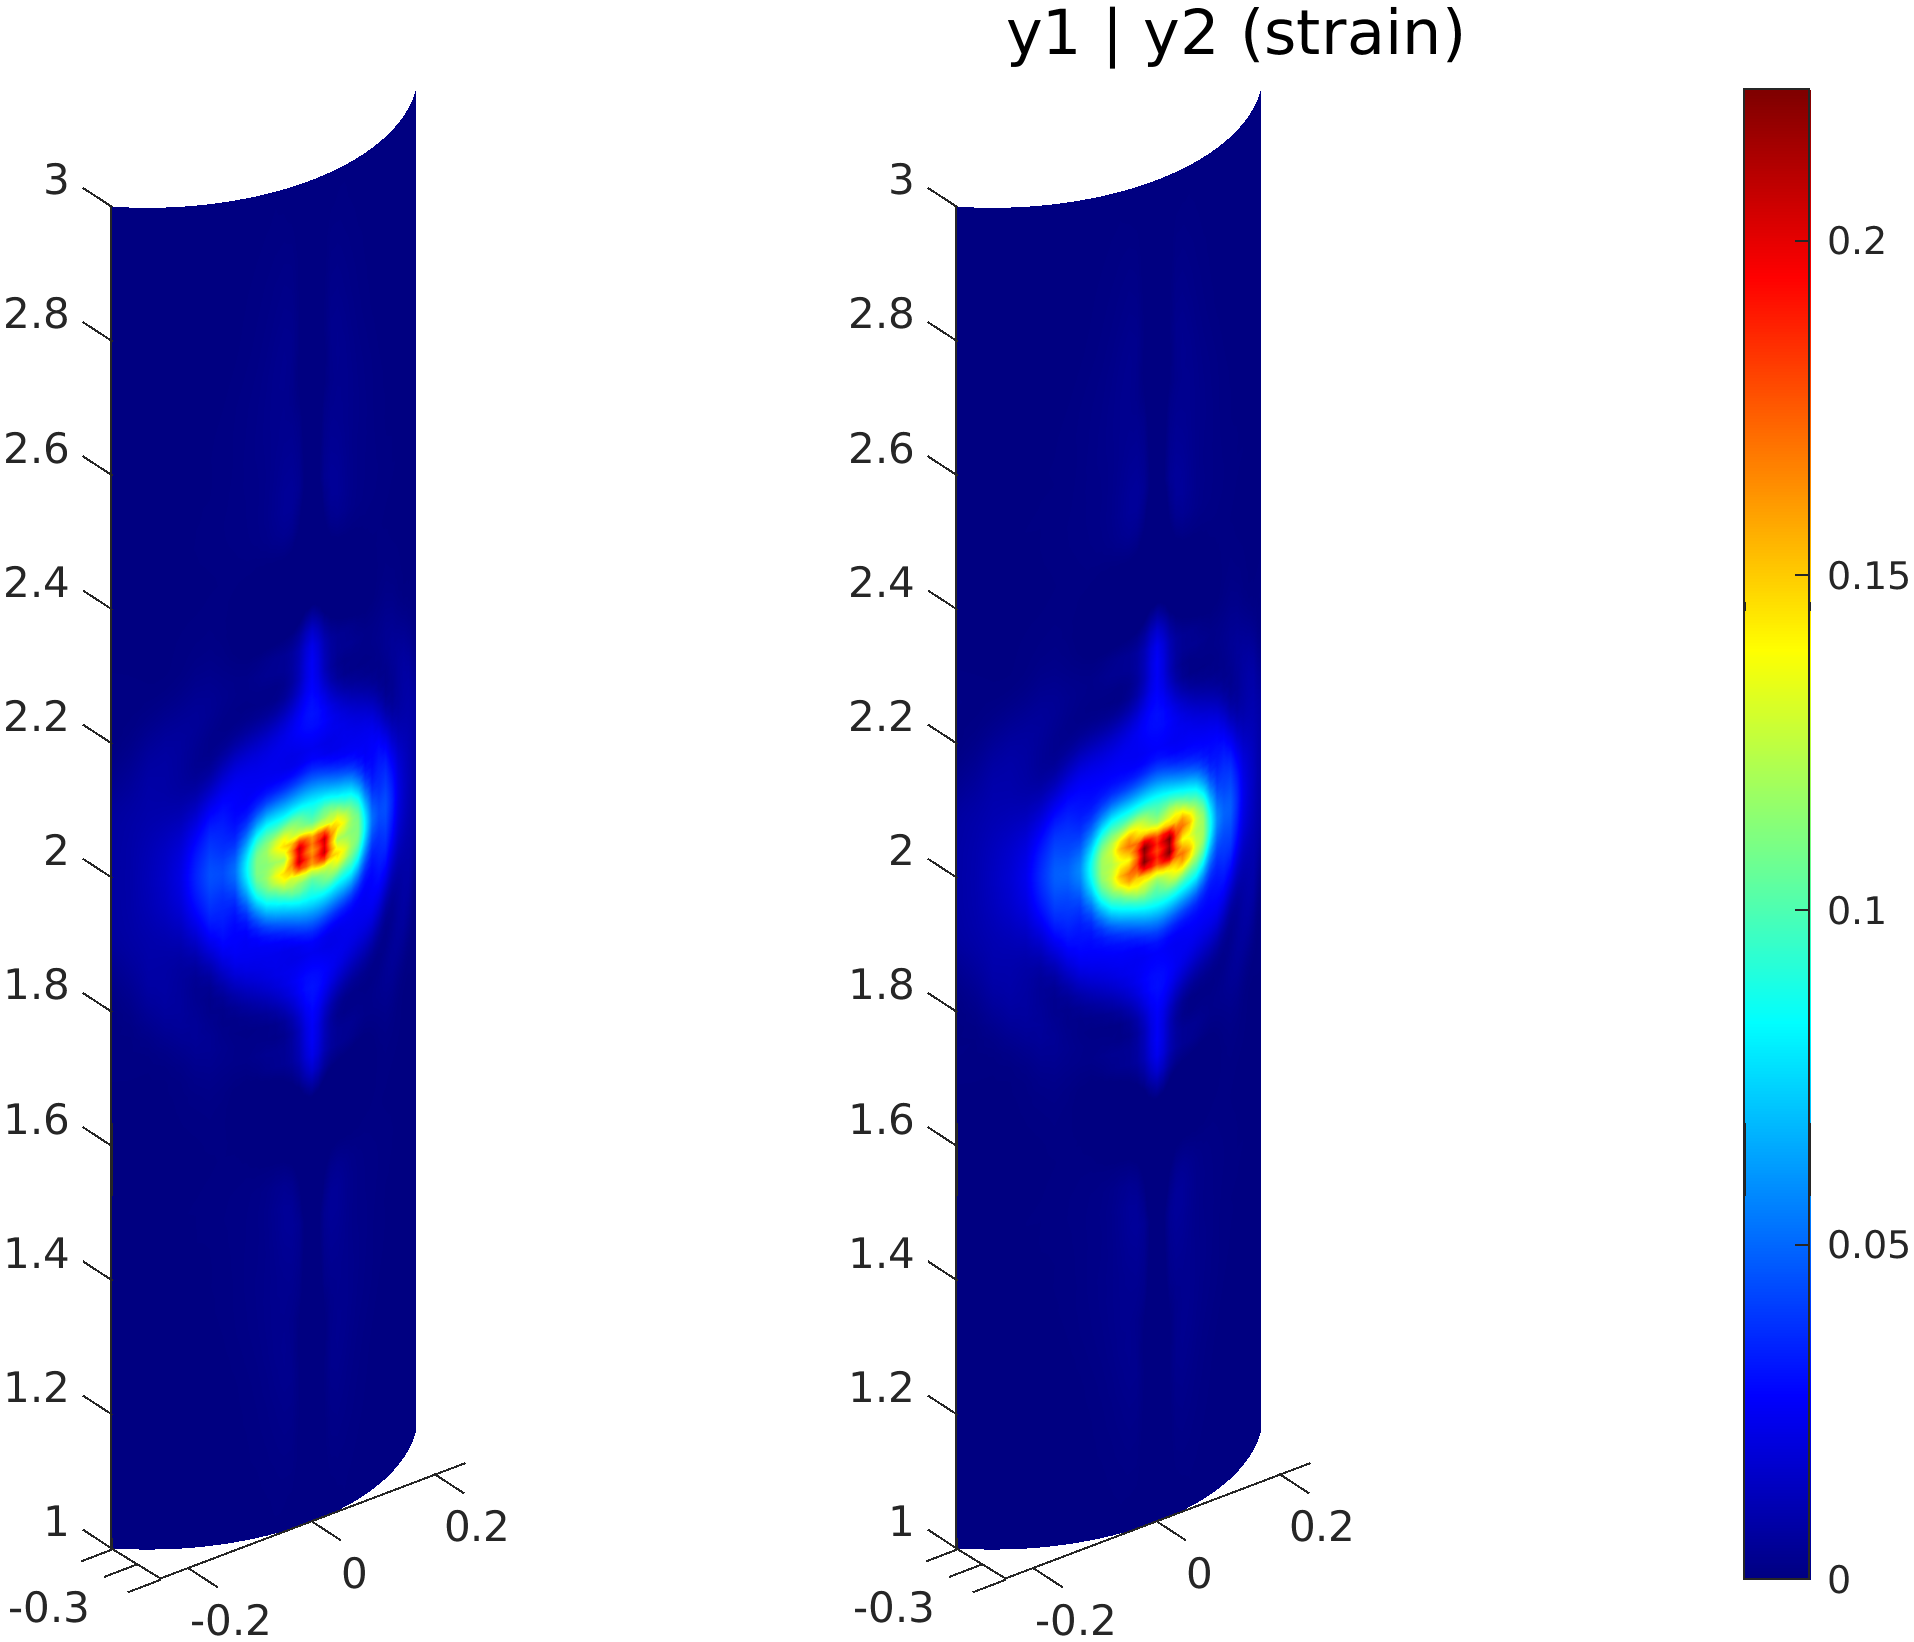
\includegraphics[scale=0.36]{strain.png}
\caption{2 slightly different deformations and their associated quite different strain as obtained by the {\em Diff} model with $200 $ binary variables.}
\vspace{-0.2cm}
\label{fig5}
\end{figure*}	

For the pipe system, we compare in Table \ref{table.pipe} the different models ITNE, {\em Diff}, {\em $2b+1$,$1b$} to produce bounds on the sum of the difference of strain over 10 specific points of the mesh, for a physically relevant perturbation of the deformation. 
The bounds we found are quite accurate, with a best bound of $.0329$ obtained by the {\em $2b+1$} model, slightly better than the bound $.0337$ found within the same time by the {\em Diff} model, and better than the bound found $.0356$ by the {\em "$1b$"} model, although this bound has been found 70 times faster due to the simpler model ({\em 1}$b$ converges after 1000s). ITNE is significantly worse than even the {\em "$1b$"} with 1000s of timeout, at $.0416$ despite a very long time out. The certified lower bound is not too far, at $.025$.

We did check that this worst-case found, displayed in Fig. \ref{fig5} and which is not too far from the actual worst case that is known to be $<0.033$, is coherent with the physical finite element model the DNN surrogate has been learned from. Hence, this brittleness of the surrogate is {\em not} a hallucination due to the learning process, but rather correctly reflects the physical system.


\section{Appendix for Section 1}

\section{Appendix for Section 2}

\section{Appendix for Section 3}

\label{app.L1}

\setcounter{proposition}{1}



\begin{proposition}
	The combine of two constraints below are equivalent with $\sum_{j\leq k} |x_j-x'_j| \leq \varepsilon$:
	
	\begin{enumerate}
		\item for all {\em input} neuron $j$ (in layer 0), 
		$A_j \geq x_j - x'_j $ and $A_j \geq x'_j - x_j$,
		
		\item $\sum_{j\leq k} A_j \leq \varepsilon$ 
		\quad \, \quad [$L_1$-perturbation $\leq \varepsilon$].
	\end{enumerate}
\end{proposition}


\begin{proof}[Proof] $\Rightarrow$ side: For any solution to the constraint $\sum_{j\leq k} |x_j-x'_j| \leq \varepsilon$, we show that it also satisfies the combined constraints. Notice that the variables $A_j$ only appear in this group of constraints. So we let $A_j = |x_j-x'_j|$ for each $j$. Then for each $j$, $A_j = |x_j-x'_j|\geq x_j - x'_j, A_j = |x_j-x'_j|\geq x'_j - x_j$,  and $$\sum_{j\leq k} A_j = \sum_{j\leq k} |x_j-x'_j| \leq\varepsilon.$$
	
	
$\Leftarrow$ side: Similarly, if solution satisfies the combined constraints, then for any $j$, we have $$A_j \geq \max\{x'_j - x_j, x_j - x'_j\} = |x_j-x'_j|.$$ Hence $$\sum_{j\leq k} |x_j-x'_j| \leq \sum_{j\leq k} A_j\leq\varepsilon.$$
\end{proof}



\section{Appendix for Section 4}



\label{app.realtime}


\begin{proposition}
	\label{Prop3}
	For all DNN and all latent space dimension $n$, $\beta^\varepsilon_{C,D}(\text{LAE-DNN}) \leq \beta^{\varepsilon}_{C,D}(\text{DNN})$.
\end{proposition}

\begin{proof}[Proof] Notice the fact that, for any input $I$ to the LAE-DNN, its the projection after encoding and decoding $I'$ is still a possible input for the original DNN, and the output is the same as the output of the original DNN given input I'.
	
Therefore the output space of LAE-DNN is a subset of the original DNN. Hence we have $\beta^\varepsilon_{C,D}(\text{LAE-DNN}) \leq \beta^{\varepsilon}_{C,D}(\text{DNN})$.
	
\end{proof}

\section{Appendix for Section 5}


\section{Appendix for Section 6}

\begin{figure}[b!]
	\centering
	%\hspace*{10ex}
	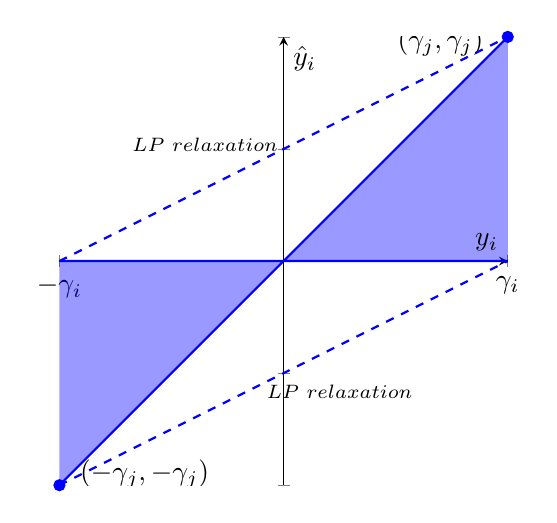
\begin{tikzpicture}
		\begin{axis}[
			xlabel={$y_i$},
			ylabel={$\hat{y}_i$},
			xmin=-2, xmax=2,
			ymin=-2, ymax=2,
			axis lines=center,
			samples=100, 
			unit vector ratio=1 1 1, scale=1, xtick   = {-2,2},
			xticklabels = {$-\gamma_i$,$\gamma_i$},
			yticklabels = {},
			]
			\addplot[blue, thick, fill=blue, fill opacity=0.4] {x} \closedcycle; 
			\addplot[blue, thick] {0}; 
			
			\addplot[only marks, mark=*, mark size=2pt, blue] coordinates {(-2,-2)};
			\node[label={above:$(-\gamma_j,-\gamma_j)$}] at (axis cs: -1.24, -2.2) {};
			
			\addplot[only marks, mark=*, mark size=2pt, blue] coordinates {(2,2)};
			\node[label={above:$(\gamma_j,\gamma_j)$}] at (axis cs: 1.4, 1.65) {};
			\addplot[dashed, thick, blue] coordinates {(-2,-2) (2,0)};
			\addplot[dashed, thick, blue] coordinates {(-2,0) (2,2)};
			\node[label={above:\scriptsize $\text{LP\ relaxation}$}] at (axis cs: -0.7, 0.8) {};
			\node[label={above:\scriptsize $\text{LP\ relaxation}$}] at (axis cs: 0.5, -1.4) {};
		\end{axis}
	\end{tikzpicture}
	\caption{Possible values of $\hat{y}_j$ depending on $y_j$ for the {\em 1b} model.}
	\label{fig.1v}
\end{figure}

\begin{proposition}
	\label{Prop4}
	Assuming $y_j \in [-\gamma_j, \gamma_j]$ and $x'_j,y_j+x'_j \in [\alpha_j,\beta_j]$, we have that $\hat{y}_j = \ReLU(x_j=y_j + x'_j) - \ReLU(x'_j)$ is the solution of the MILP program:
	\begin{align*}
		& \begin{aligned}
			y_j + x'_j &\leq a\beta_j        &
			y_j &+ x'_j \geq (1-a)\alpha_j \\
			x'_j       &\leq a'\beta_j       & 
			x'_j       &\geq (1-a')\alpha_j \\
			\hat{y}_j  &\leq a\gamma_j       &
			\hat{y}_j  &\geq -a'\gamma_j \\
			\hat{y}_j  &\leq y_j + x'_j - (1-a)\alpha_j &
			\hat{y}_j  &\geq y_j + x'_j - a'\beta_j \\
			\hat{y}_j  &\leq -x'_j + a\beta_j &
			\hat{y}_j  &\geq -x'_j + (1-a')\alpha_j \\
			\hat{y}_j  &\leq y_j + (1-a)\gamma_j  &
			\hat{y}_j  &\geq y_j - (1-a')\gamma_j
		\end{aligned}
	\end{align*} 
	where $a,a' \in \{0,1\}$ are binary variables, 
	and $a'$ is shared with the classical MILP
	encoding for $\hat{x}'_j=\ReLU(x'_j)$.
\end{proposition}

\begin{proof}[Proof]
	First, we list the inequalities: \begin{align*}
		& \begin{aligned}
			y_j + x'_j &\leq a\beta_j        &
			y_j &+ x'_j \geq (1-a)\alpha_j \\
			x'_j       &\leq a'\beta_j       & 
			x'_j       &\geq (1-a')\alpha_j \\
			\hat{y}_j  &\leq a\gamma_j       &
			\hat{y}_j  &\geq -a'\gamma_j \\
			\hat{y}_j  &\leq y_j + x'_j - (1-a)\alpha_j &
			\hat{y}_j  &\geq y_j + x'_j - a'\beta_j \\
			\hat{y}_j  &\leq -x'_j + a\beta_j &
			\hat{y}_j  &\geq -x'_j + (1-a')\alpha_j \\
			\hat{y}_j  &\leq y_j + (1-a)\gamma_j  &
			\hat{y}_j  &\geq y_j - (1-a')\gamma_j
		\end{aligned}
	\end{align*} 
	
	Follow the discuss in the proof of main text, we need to check the other inequalities of each cases.
	
 \textbf{$\mathbf{a = 0, a' = 0}$:}  In this case, the inequalities become: \begin{align*}
 	& \begin{aligned}
 		y_j + x'_j &\leq 0       &
 		y_j &+ x'_j \geq \alpha_j \\
 		x'_j       &\leq 0       & 
 		x'_j       &\geq \alpha_j \\
 		\hat{y}_j  &\leq 0       &
 		\hat{y}_j  &\geq 0 \\
 		\hat{y}_j  &\leq y_j + x'_j -\alpha_j &
 		\hat{y}_j  &\geq y_j + x'_j  \\
 		\hat{y}_j  &\leq -x'_j  &
 		\hat{y}_j  &\geq -x'_j + \alpha_j \\
 		\hat{y}_j  &\leq y_j + \gamma_j  &
 		\hat{y}_j  &\geq y_j - \gamma_j
 	\end{aligned}
 \end{align*} Now we can see, $y_j+x'_j\leq 0$ and $x'_j \leq 0$ (lines 1\&2), $\hat{y}_j=0$ (line 3). 
 
 For other 3 lines, by above discussing and the assumption of the proposition that $y_j \in [-\gamma_j, \gamma_j]$ and $x'_j,y_j+x'_j \in [\alpha_j,\beta_j]$, they are implied by the following inequalities respectively (one for one) \begin{align*}
 & \begin{aligned}
 	\hat{y}_j  \leq 0 &\leq y_j + x'_j -\alpha_j &
 	\hat{y}_j  \geq 0 &\geq y_j + x'_j  \\
 	\hat{y}_j  \leq 0 &\leq -x'_j  &
 	\hat{y}_j  \geq 0 &\geq -x'_j + \alpha_j \\
 	\hat{y}_j  \leq 0 &\leq y_j + \gamma_j  &
 	\hat{y}_j  \geq 0 &\geq y_j - \gamma_j
 \end{aligned}
 \end{align*} Therefore all 3 rest lines are implied by other inequalities.
 
 
\textbf{$\mathbf{a = 1, a' = 0}$:} In this case, the inequalities become: \begin{align*}
	& \begin{aligned}
		y_j + x'_j &\leq \beta_j        &
		y_j &+ x'_j \geq 0 \\
		x'_j       &\leq 0       & 
		x'_j       &\geq \alpha_j \\
		\hat{y}_j  &\leq \gamma_j       &
		\hat{y}_j  &\geq 0 \\
		\hat{y}_j  &\leq y_j + x'_j &
		\hat{y}_j  &\geq y_j + x'_j  \\
		\hat{y}_j  &\leq -x'_j + \beta_j &
		\hat{y}_j  &\geq -x'_j + \alpha_j \\
		\hat{y}_j  &\leq y_j  &
		\hat{y}_j  &\geq y_j - \gamma_j
	\end{aligned}
\end{align*} Now we can see, $y_j+x'_j\geq 0$ and $x'_j \leq 0$ (lines 1\&2), hence $y_j \geq 0$; and $\hat{y}_j= y_j + x'_j$ (line 4). 

By above discussing,  we have: \begin{align*}
	& \begin{aligned}
		\hat{y}_j  \leq& y_j+x'_j \leq y_j  &\hat{y}_j  \geq& y_j+x'_j \geq 0
	\end{aligned}
\end{align*}

Then by the assumption of the proposition that $y_j \in [-\gamma_j, \gamma_j]$ and $x'_j,y_j+x'_j \in [\alpha_j,\beta_j]$, all 3 other lines are implied by the following inequalities respectively (one for one): \begin{align*}
	& \begin{aligned}
		\hat{y}_j  \leq&  y_j \leq \gamma_j       &
		\hat{y}_j  \geq& y_j+x'_j \geq 0 \\
		\hat{y}_j  \leq& 0 \leq -x'_j + \beta_j &
		\hat{y}_j  \geq& 0 \geq -x'_j + \alpha_j \\
		\hat{y}_j  \leq& y_j+x'_j \leq y_j  &
		\hat{y}_j  \geq& 0 \geq y_j - \gamma_j
	\end{aligned}
\end{align*}Therefore all 3 rest lines are implied by other inequalities.
	

	
\textbf{$\mathbf{a = 0, a' = 1}$:}  In this case, the inequalities become: \begin{align*}
	& \begin{aligned}
		y_j + x'_j &\leq 0        &
		y_j &+ x'_j \geq \alpha_j \\
		x'_j       &\leq \beta_j       & 
		x'_j       &\geq 0 \\
		\hat{y}_j  &\leq 0      &
		\hat{y}_j  &\geq -\gamma_j \\
		\hat{y}_j  &\leq y_j + x'_j - \alpha_j &
		\hat{y}_j  &\geq y_j + x'_j  -\beta_j\\
		\hat{y}_j  &\leq -x'_j &
		\hat{y}_j  &\geq -x'_j \\
		\hat{y}_j  &\leq y_j + \gamma_j  &
		\hat{y}_j  &\geq y_j
	\end{aligned}
\end{align*} Now we can see, $y_j+x'_j\leq 0$ and $x'_j \geq 0$ (lines 1\&2), hence $y_j \leq 0$; and $\hat{y}_j= - x'_j$ (line 5). 

By above discussing,  we have: \begin{align*}
	& \begin{aligned}
		\hat{y}_j  &\leq -x'_j\leq 0      & \hspace*{4ex}
		\hat{y}_j  &\geq -x'_j \geq -x'_j+(y_j+x'_j) \geq y_j
	\end{aligned}
\end{align*}

Then by the assumption of the proposition that $y_j \in [-\gamma_j, \gamma_j]$ and $x'_j,y_j+x'_j \in [\alpha_j,\beta_j]$, all 3 other lines are implied by the following inequalities respectively (one for one):\begin{align*}
	& \begin{aligned}
		\hat{y}_j  &\leq -x'_j\leq 0      &
		\hat{y}_j  &\geq y_j\geq -\gamma_j \\
		\hat{y}_j  &\leq 0 \leq y_j + x'_j - \alpha_j &
		\hat{y}_j  &\geq y_j \geq y_j + x'_j -\beta_j \\
		\hat{y}_j  &\leq 0 \leq y_j + \gamma_j  &
		\hat{y}_j  &\geq  y_j
	\end{aligned}
\end{align*}Therefore all 3 rest lines are implied by other inequalities.




	
\textbf{$\mathbf{a = 1, a' = 1}$:} In this case, the inequalities become: \begin{align*}
	& \begin{aligned}
		y_j + x'_j &\leq \beta_j        &
		y_j &+ x'_j \geq 0 \\
		x'_j       &\leq \beta_j       & 
		x'_j       &\geq 0 \\
		\hat{y}_j  &\leq \gamma_j       &
		\hat{y}_j  &\geq -\gamma_j \\
		\hat{y}_j  &\leq y_j + x'_j  &
		\hat{y}_j  &\geq y_j + x'_j - \beta_j \\
		\hat{y}_j  &\leq -x'_j + \beta_j &
		\hat{y}_j  &\geq -x'_j \\
		\hat{y}_j  &\leq y_j &
		\hat{y}_j  &\geq y_j
	\end{aligned}
\end{align*} Now we can see, $y_j+x'_j\geq 0$ and $x'_j \geq 0$ (lines 1\&2) and $\hat{y}_j= y_j$ (line 6). 


Then by the assumption of the proposition that $y_j \in [-\gamma_j, \gamma_j]$ and $x'_j,y_j+x'_j \in [\alpha_j,\beta_j]$, all 3 other lines are implied by the following inequalities respectively (one for one):\begin{align*}
	& \begin{aligned}
		\hat{y}_j  &\leq y_j\leq \gamma_j       &
		\hat{y}_j  &\geq y_j\geq -\gamma_j \\
		\hat{y}_j  &\leq y_j \leq y_j + x'_j  &
		\hat{y}_j  &\geq y_j \geq y_j + x'_j - \beta_j \\
		\hat{y}_j  &\leq -x'_j+(y_j+x'_j)\leq -x'_j + \beta_j &
		\hat{y}_j  &\geq y_j - (y_j+x'_j)\geq -x'_j \\
	\end{aligned}
\end{align*}Therefore all 3 rest lines are implied by other inequalities.
	

\end{proof}

  \begin{proposition}
	\label{prop5}
	Given $y_i \in [-\gamma_i,\gamma_i]$, 
	$\hat{y}_i$ is a solution of the MILP program :\begin{align*}
		\hat{y}_i &\leq a \gamma_i               &\quad \hat{y}_i &\geq y_i - a \gamma_i \\
		\hat{y}_i &\geq (a-1) \gamma_i           &\quad \hat{y}_i &\leq y_i + (1-a) \gamma_i
	\end{align*} where $a \in \{0,1\}$ is a binary variable.
\end{proposition}

\begin{proof}[Proof] First, we list the inequalities: \begin{align*}
		\hat{y}_i &\leq a \gamma_i               &\quad \hat{y}_i &\geq y_i - a \gamma_i \\
		\hat{y}_i &\geq (a-1) \gamma_i           &\quad \hat{y}_i &\leq y_i + (1-a) \gamma_i
	\end{align*}
	
	Similar to Proposition 4, we consider by cases.
	
	\textbf{$\mathbf{a = 0}$:} In this case, the inequalities become: \begin{align*}
		\hat{y}_i &\leq 0               &\quad \hat{y}_i &\geq y_i \\
		\hat{y}_i &\geq -\gamma_i           &\quad \hat{y}_i &\leq y_i + \gamma_i
	\end{align*} Now we can see, $y_i\leq 0$ (line 1) and $y_i\leq\hat{y}_i\leq 0 $. Line 2 is implied by other inequalities since \begin{align*}
	\hat{y}_i &\geq y_i \geq -\gamma_i           &\quad \hat{y}_i &\leq 0 \leq y_i + \gamma_i
	\end{align*}

	\textbf{$\mathbf{a = 1}$:} In this case, the inequalities become: \begin{align*}
		\hat{y}_i &\leq \gamma_i               &\quad \hat{y}_i &\geq y_i - \gamma_i \\
		\hat{y}_i &\geq 0           &\quad \hat{y}_i &\leq y_i 
	\end{align*} Now we can see, $y_i\geq 0$ (line 2) and $0\leq\hat{y}_i\leq y_i $. Line 1 is implied by other inequalities since \begin{align*}
	\hat{y}_i &\leq y_i\leq \gamma_i               &\quad \hat{y}_i &\geq 0 \geq y_i - \gamma_i 
	\end{align*}
		
Now we finish the proof. 
\end{proof}


\section{Appendix for Section 7}


\section{NeurIPS Paper Checklist}



\begin{enumerate}
	
	\item {\bf Claims}
	\item[] Question: Do the main claims made in the abstract and introduction accurately reflect the paper's contributions and scope?
	\item[] Answer: \answerYes{} % Replace by \answerYes{}, \answerNo{}, or \answerNA{}.
	\item[] Justification: The claims of (3-15x), DiffMILP and online is in the section of experiments. LAE is explained in Section 5 and DiffMILP is explained in Section 6.

	
	\item {\bf Limitations}
	\item[] Question: Does the paper discuss the limitations of the work performed by the authors?
	\item[] Answer: \answerYes{} % Replace by \answerYes{}, \answerNo{}, or \answerNA{}.
	\item[] Justification: As we said in the introduction, our techniques are tested on several DNNs and datasets, but DNN size is limited (though concrete examples are tackled). 
	Linear AE and Linear and ReLU activation functions are the ones we experimented on. 

	
	\item {\bf Theory assumptions and proofs}
	\item[] Question: For each theoretical result, does the paper provide the full set of assumptions and a complete (and correct) proof?
	\item[] Answer: \answerYes{} % Replace by \answerYes{}, \answerNo{}, or \answerNA{}.
	\item[] Justification: The full proofs of propositions appear in the supplemental material (appendix).

	
	\item {\bf Experimental result reproducibility}
	\item[] Question: Does the paper fully disclose all the information needed to reproduce the main experimental results of the paper to the extent that it affects the main claims and/or conclusions of the paper (regardless of whether the code and data are provided or not)?
	\item[] Answer: \answerYes{} % Replace by \answerYes{}, \answerNo{}, or \answerNA{}.
	\item[] Justification: The whole process of the method and all datasets, models and hyperparameters are clearly stated in Section 5, 6, and 7.

	
	
	\item {\bf Open access to data and code}
	\item[] Question: Does the paper provide open access to the data and code, with sufficient instructions to faithfully reproduce the main experimental results, as described in supplemental material?
	\item[] Answer: \answerNo{} % Replace by \answerYes{}, \answerNo{}, or \answerNA{}.
	\item[] Justification: We will release the code in the near future.

	
	
	\item {\bf Experimental setting/details}
	\item[] Question: Does the paper specify all the training and test details (e.g., data splits, hyperparameters, how they were chosen, type of optimizer) necessary to understand the results?
	\item[] Answer: \answerYes{} % Replace by \answerYes{}, \answerNo{}, or \answerNA{}.
	\item[] Justification: All datasets, models and hyperparameters are clearly stated.

	
	\item {\bf Experiment statistical significance}
	\item[] Question: Does the paper report error bars suitably and correctly defined or other appropriate information about the statistical significance of the experiments?
	\item[] Answer:\answerNo{} % Replace by \answerYes{}, \answerNo{}, or \answerNA{}.
	\item[] Justification: There is no error bars appear in the paper.

	
	\item {\bf Experiments compute resources}
	\item[] Question: For each experiment, does the paper provide sufficient information on the computer resources (type of compute workers, memory, time of execution) needed to reproduce the experiments?
	\item[] Answer: \answerYes{} % Replace by \answerYes{}, \answerNo{}, or \answerNA{}.
	\item[] Justification: The required information is provided at the beginning of the experimental section.

	
	\item {\bf Code of ethics}
	\item[] Question: Does the research conducted in the paper conform, in every respect, with the NeurIPS Code of Ethics \url{https://neurips.cc/public/EthicsGuidelines}?
	\item[] Answer: \answerYes{} % Replace by \answerYes{}, \answerNo{}, or \answerNA{}.
	\item[] Justification: The paper complies with the NeurIPS Code of Ethics. The proposed work does not involve human subjects, crowdsourcing, or sensitive data, and therefore does not raise any of the ethical concerns described in the guidelines.

	
	
	\item {\bf Broader impacts}
	\item[] Question: Does the paper discuss both potential positive societal impacts and negative societal impacts of the work performed?
	\item[] Answer: \answerNA{} % Replace by \answerYes{}, \answerNo{}, or \answerNA{}.
	\item[] Justification: The work presents a theoretical framework. It does not involve data collection from individuals or system deployment, and therefore does not introduce foreseeable negative societal impacts such as privacy, fairness, or security risks.

	
	\item {\bf Safeguards}
	\item[] Question: Does the paper describe safeguards that have been put in place for responsible release of data or models that have a high risk for misuse (e.g., pre-trained language models, image generators, or scraped datasets)?
	\item[] Answer: \answerNA{} % Replace by \answerYes{}, \answerNo{}, or \answerNA{}.
	\item[] Justification: This paper does not release any data or models that pose a risk.

	
	\item {\bf Licenses for existing assets}
	\item[] Question: Are the creators or original owners of assets (e.g., code, data, models), used in the paper, properly credited and are the license and terms of use explicitly mentioned and properly respected?
	\item[] Answer: \answerYes{} % Replace by \answerYes{}, \answerNo{}, or \answerNA{}.
	\item[] Justification: The original owners of assets code, data, models used in the paper are properly credited. The license and terms of use explicitly are mentioned and properly respected.
	\item[] Guidelines:
	
	
	\item {\bf New assets}
	\item[] Question: Are new assets introduced in the paper well documented and is the documentation provided alongside the assets?
	\item[] Answer: \answerNA{} % Replace by \answerYes{}, \answerNo{}, or \answerNA{}.
	\item[] Justification: The paper does not release new assets.
	
	
	\item {\bf Crowdsourcing and research with human subjects}
	\item[] Question: For crowdsourcing experiments and research with human subjects, does the paper include the full text of instructions given to participants and screenshots, if applicable, as well as details about compensation (if any)? 
	\item[] Answer: \answerNA{} % Replace by \answerYes{}, \answerNo{}, or \answerNA{}.
	\item[] Justification: The paper does not involve crowdsourcing nor research with human subjects.

	
	\item {\bf Institutional review board (IRB) approvals or equivalent for research with human subjects}
	\item[] Question: Does the paper describe potential risks incurred by study participants, whether such risks were disclosed to the subjects, and whether Institutional Review Board (IRB) approvals (or an equivalent approval/review based on the requirements of your country or institution) were obtained?
	\item[] Answer: \answerNA{} % Replace by \answerYes{}, \answerNo{}, or \answerNA{}.
	\item[] Justification: The paper does not involve crowdsourcing nor research with human subjects.
	
	
	\item {\bf Declaration of LLM usage}
	\item[] Question: Does the paper describe the usage of LLMs if it is an important, original, or non-standard component of the core methods in this research? Note that if the LLM is used only for writing, editing, or formatting purposes and does \emph{not} impact the core methodology, scientific rigor, or originality of the research, declaration is not required.
	%this research? 
	\item[] Answer: \answerNA{} % Replace by \answerYes{}, \answerNo{}, or \answerNA{}.
	\item[] Justification: The core method development in this research does not involve LLMs as any important, original, or non-standard components.
\end{enumerate}



%\section{A table comparing PCA and FULL}
%
%
%
%	\begin{table}[b!]
%	\centering
%	\begin{tabular}{|c|c||c|c||c|}\hline
%		Network & Norm & Full& PCA &  Ratio \\\hline \hline 
%		MNIST-FC  & $L_1$ & 33.68 & 2.00  & {\bf 16.84$\times$}\\\hline
%		MNIST-FC  & $L_\infty$ & 180.73 & 66.11 & {\bf 2.73$\times$} \\\hline\hline
%		
%		MNIST-Conv1  & $L_1$ & 3.24 & 1.16 & {\bf 2.79$\times$}\\\hline
%		MNIST-Conv1  & $L_\infty$ & 1.96 & 0.83 & {\bf 2.36 $\times$}\\\hline\hline
%	
%		
%		FMNIST-Conv1  & $L_1$ & 6.37& 1.95   & {\bf 3.27$\times$}\\\hline
%		FMNIST-Conv1 & $L_\infty$ & 2.44& 1.36   & {\bf 1.79$\times$} \\\hline\hline
%		
%		CIFAR-10-Conv1  & $L_1$ &7.19 & 1.15 &  {\bf 6.25$\times$} \\\hline
%		CIFAR-10-Conv1  & $L_\infty$ & 4.33 & 1.24   & {\bf 3.49 $\times$} \\\hline\hline
%
%	\end{tabular}
%	\caption{
%	}
%\end{table}
